\subsubsection{Part 2:}

Within the wifi-example-sim.cc file, the transmission bitrate can be modified in
one of two ways. By modifying the size of the packets being transmit, or by
modifying the delay between packet transmissions. This is shown in the following
calculations:

\begin{gather*}
	R=\frac{rxPackets\times packetSize \times 8}{txTime} \\
	\begin{align*}
		\frac{R\times txTime}{packetSize \times 8} &= rxPackets &
		\undeline{or}& & \frac{R \times txTime}{rxPackets
	\times 8} &= packetSize \\
	\end{align*} \\
	rxPackets=\frac{txTime}{delay}
\end{gather*}
\captionof{equation}{Calculation for Bitrate Modification}

The following table shows the number of packets to be sent (modified by the
delay between packet transmissions), or the size of packet to be sent in order
to meet the required data rates.

\begin{table}[H]
	\centering
	\caption{Bitrate Calculation Results}
	\label{tab:brcalc}
	\begin{tabular}{|c|c|c|c|}
	\hline
	Bitrate & rxPackets & Delay & packetSize \\
	\hline
	1Mbps & 2,500 & $8\times 10^{-3}$ & 625 \\
	1.5Mbps & 3,750 & $5.3\times 10^{-3}$ & 937.5 \\
	5Mbps & 12,500 & $1.6\times 10^{-3}$ & 3125 \\
	10Mbps & 25,000 & $8\times 10^{-4}$ & 6250 \\
	20Mbps & 50,000 & $4\times 10^{-4}$ & 12,500 \\
	\hline
	\end{tabular}
\end{table}

For the purposes of this section, the delay between the packet transmissions
will be modified. Modifying packet sizes requires using half bytes for packet
sizes.

\par The following equations show the throughput, delay, and packet loss ratio
for the systems with the above bitrates.

\begin{gather*}
	Throughput=\frac{rxPackets*1000*8}{txTime} \\
	TP_{8\times10^{-3}}=\frac{2500*1000*8}{20} \\
	= 1000Kbps \\
	TP_{5.3\times10^{-3}}=\frac{3774*1000*8}{20} \\
	= 1509.6Kbps \\
	TP_{1.6\times10^{-3}}=\frac{12500*1000*8}{20} \\
	= 5000Kbps \\
	TP_{8\times10^{-4}}=\frac{24997*1000*8}{20} \\
	= 9998.8Kbps \\
	TP_{4\times10^{-4}}=\frac{34368*1000*8}{20} \\
	= 13747.2Kbps
\end{gather*}
\captionof{equation}{Average Throughput (Kbps}

\par From these calculations, it can be seen that a maximum throughput of
13.7Mbps was achieved. Loss begins to occur at approximately 10Mbps, limiting
the throughput. The throughput can be seen plotted against the increasing
transmission intervals in Figure \ref{fig:QAP2Throughput}

\begin{figure}[H]
	\centering
	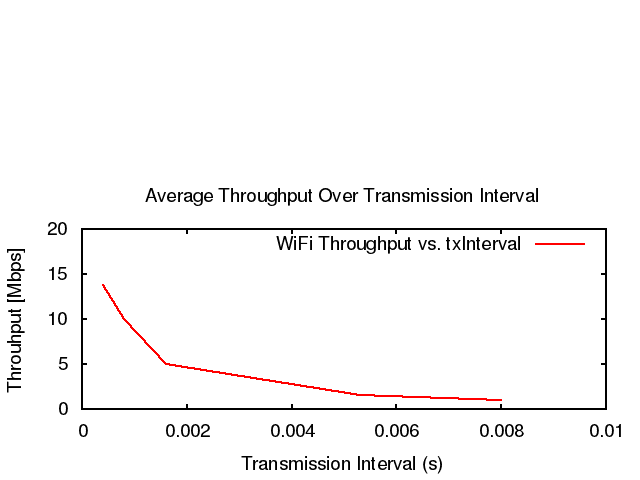
\includegraphics[width=0.8\textwidth]{images/EE500/QA/P2/Images/wifi-throughput}
	\caption{Throughput for transmission intervals as outlined in
	Table \ref{tab:brcalc}}
	\label{fig:QAP2Throughput}
\end{figure}

\begin{gather*}
	\overline{delay}=\frac{delaySum}{rxPackets} \\
\overline{delay}_{8\times10^{-3}}=\frac{1102533332}{2500} \\
	= 441013.3328ns \\
	\overline{delay}_{5.3\times10^{-3}}=\frac{1649679480}{3774} \\
	= 437116.9793ns \\
	\overline{delay}_{1.6\times10^{-3}}=\frac{5484597352}{12500} \\
	= 438767.7882ns \\
	\overline{delay}_{8\times10^{-4}}=\frac{12434305114}{24497} \\
	= 497431.8964ns \\
	\overline{delay}_{4\times10^{-4}}=\frac{7873637069728}{34368} \\
	= 229097912.9ns \\
\end{gather*}
\captionof{equation}{Average Delay (s)}

\par These calculations show that there is an increase in delay as the bitrate
increases (i.e. the transmission interval decreases). This is further
demonstrated in Figure \ref{fig:QAP2Delay}.

\begin{figure}[H]
	\centering
	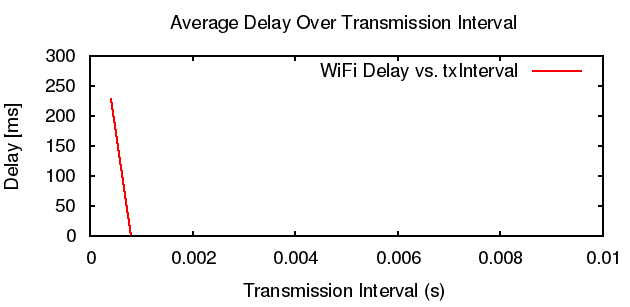
\includegraphics[width=0.8\textwidth]{images/EE500/QA/P2/Images/wifi-delay}
	\caption{Delay for transmission intervals as outlined in Table
	\ref{tab:brcalc}}
	\label{fig:QAP2Delay}
\end{figure}

\begin{gather*}
	PLR=\frac{lostPackets}{rxPackets+lostPackets} \\
	PLR_{8\times10^{-3}}=\frac{0}{2500+0} \\
	= 0 \\
	PLR_{5.3\times10^{-3}}=\frac{0}{3774+0} \\
	= 0 \\
	PLR_{1.6\times10^{-3}}=\frac{0}{12500+0} \\
	= 0 \\
	PLR_{8\times10^{-4}}=\frac{3}{24997+3} \\
	= 1.2\times10^{-4} \\
	PLR_{4\times10^{-4}}=\frac{15632}{34368+15632} \\
	= 0.30724
\end{gather*}
\captionof{equation}{Average Packet Loss Ratio}

Again, as there is an increase in the bitrate, there is an increase in the loss
within the system, with a maximum loss of 30\%, which can be clearly seen within
Figure \ref{fig:QAP2Loss}.

\begin{figure}[H]
	\centering
	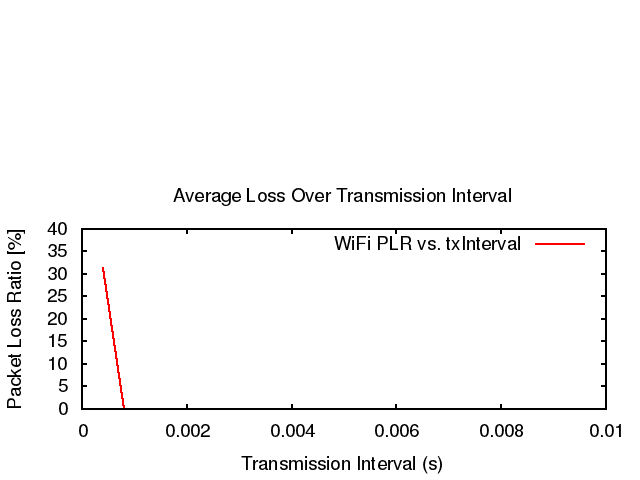
\includegraphics[width=0.8\textwidth]{images/EE500/QA/P2/Images/wifi-loss}
	\caption{Loss for transmission intervals as outlined in Table
	\ref{tab:brcalc}}
	\label{fig:QAP2Loss}
\end{figure}

This section displays clearly that there is a direct relation between the
bitrate and the throughput, delay, and loss. As the bitrate was increased in
each test case, the throughput increased, until the point at which the loss and
delay began to affect the linearity of the increase.
